\chapter{Spiking classification on large multi-subject P300 dataset} \label{chap:06}

A convolutional neural network described in \cite{varekaEvaluationConvolutional20} was converted with the SNN conversion toolbox. SNN-TB was selected for the conversion over Nengo simulation platform because the CNN contained batch normalisation layer and softmax activation function, which prevented Nengo to convert the network successfully. \par
The original CNN was used for binary classification of event-related potential (ERP) signals retrieved from large multi-subject P300 dataset, which was presented in \cite{moucekEventrelatedPotential17}. The dataset was retrieved from EEG experiments, where subjects were told to concentrate on a single-digit number (from 0 to 9). Experimenters were trying to guess the number, which the subject selected, from recorded EEG data while the subject was stimulated with random sequences of all digits. It is described in \cite{varekaEvaluationConvolutional20} how were extracted short intervals of signal around all target stimuli from this dataset. An equal amount of non-target samples was acquired randomly from the remaining data. This newly-emerged dataset consisted of two distinct equal-sized classes, the target epochs (i.e. short time intervals of EEG data around the stimulus, which was the subject's thought number) and the non-target epochs. Each epoch contained three EEG channels and was 1200 ms long. The sampling frequency was 1 kHz. That means that each sample of the network input was a $3 \times 1200$ matrix. \par
The input data were preprocessed in a similar fashion as in \cite{varekaEvaluationConvolutional20}. A modified subset \cite{moucekReplicationData19} of the original dataset was used for this work. This dataset was created during the classification with the original CNN. The input file contained one matrix of feature vectors for all target data and one matrix of feature vectors for all non-target data. Those matrices were concatenated to create the input vectors. The corresponding ground truth labels were produced by one-hot-encoding of the input data. Then, severely damaged epochs were discarded from the input the same way as in the original article \cite{varekaEvaluationConvolutional20}. It was done by discarding all epochs, where amplitudes were higher than 100 $\mu V$ in any of the three channels. The steps of preprocessing is visualised in \cref{fig:gtn_preprocessing}.

\begin{figure}[htb]
    \centering
    \includesvg[inkscapelatex=false,width=\linewidth]{gtn_preprocessing}
    \caption{Flow of data preprocessing.}
    \label{fig:gtn_preprocessing}
\end{figure}

These preprocessed data were divided into training and test subsets by randomly picking out 25\% of the dataset samples into the test set. The test set was saved to the file system so it could be passed to SNN-TB during conversion later. \par
The network architecture of the CNN model was replicated entirely from the original work. This model was cross-validated the same way as in the original article. That means 30 iterations of the Monte-Carlo cross-validation were performed, and each iteration held out 25\% of the training set to create validation subset. In each iteration, a new instance of the network was created and trained. The training was done in 30 epochs while early stopping with patience value of 5 was used. After that, the trained ANN was evaluated on the test set. 10\% of the dataset samples, which were used during the training, were saved for normalisation of the layer weights. SNN-TB did this normalisation before the conversion process. All the divisions of the dataset are shown in \cref{fig:gtn_data_spliting}.

\begin{figure}[htb]
    \centering
    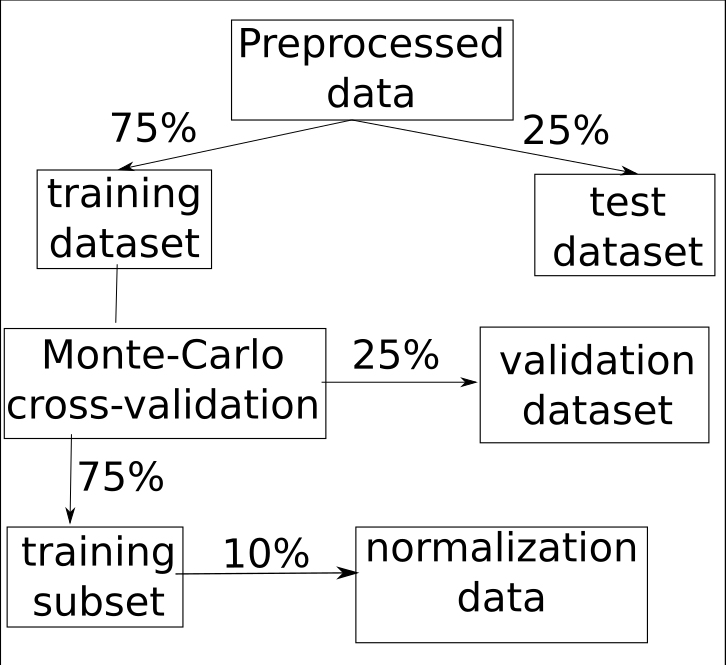
\includegraphics[width=\linewidth]{gtn_data_splitting}
    \caption{Data splitting. Proportions of the split are marked by percentages along the edges.}
    \label{fig:gtn_data_spliting}
\end{figure}

The conversion toolbox parsed the evaluated ANN into its internal Keras representation, weights of the parsed model were normalised with previously saved part of the training data. The normalised model was converted into a spiking model, and the spiking model was evaluated on the test set each iteration. The evaluation of each input sample of the spiking network was simulated for 50 timesteps. The simulator evaluated the whole test set gradually in batches of 49 samples. \par
Accuracies from the 30 iterations of cross-validation were recorded for both networks. The other metrics, which are shown in the article about the original neural network (AUC, precision, recall), could not be computed, because SNN-TB does not provide a simple way to define arbitrary metrics at this time \footnotemark.

\footnotetext{This issue was discussed with a contributor to the SNN conversion toolbox on the project's GitHub page. The discussion did not lead to a successful implementation of the custom metrics before this work was completed. A link to the website \url{https://github.com/NeuromorphicProcessorProject/snn_toolbox/issues/56} is provided with a hope that the solution might appear there in future.}

\section{Results}
The average accuracy and sample standard deviation from the 30 cross-validation iterations of the experiment are shown in \cref{tab:GTN_results}. \Cref{fig:GTN_graph} shows a comparison of the accuracies from the individual iterations. The decrease of accuracy on the SNN was expected as previous works from the field reports similar drops of performance. Also, this experiment validated only a single combination of network parameters, which is stated in the previous section. There are plenty of parameters (for the used neuron type, network or the whole simulator), so there surely is a space for fine-tuning and optimization. Whole other area of experimentation would appear if the SNN-TB was used with any other supported backend. That would possibly allow using other neuron types.

\begin{table}[htbp]
    \centering
    \begin{tabularx}{\linewidth}{>{\raggedright\arraybackslash}Xcc}
    \toprule
        Model & Average test accuracy & Sample standard deviation \\
    \midrule
        Original model & 0.6370 & 0.0066 \\
        Converted model & 0.5720 & 0.0156 \\
    \bottomrule
    \end{tabularx}
    \caption{Average accuracy and sample standard deviation of the classification results received during cross-validation.}
    \label{tab:GTN_results}
\end{table}

\begin{figure}[htbp]
    \centering
    \includesvg[width=\linewidth]{GTN_graph}
    \caption{The accuracies across all iterations of the experiment.}
    \label{fig:GTN_graph}
\end{figure}






